% Slides for the discussion with the supervisor. Compile with pdflatex (two runs).
% Every number has its source file in a comment; paths are relative to the repository root.
\documentclass[aspectratio=169,11pt]{beamer}
\usepackage[T1]{fontenc}
\usepackage[utf8]{inputenc}
\usepackage{lmodern}
\usepackage{booktabs}
\usepackage{array}
\usepackage{tikz}
\usetikzlibrary{arrows.meta,positioning,fit,calc,backgrounds}

% ---------------------------------------------------------------- theme
\usetheme{default}
\setbeamertemplate{navigation symbols}{}
\definecolor{accent}{RGB}{155,0,20}
\definecolor{muted}{RGB}{110,110,110}
\setbeamercolor{frametitle}{fg=accent}
\setbeamercolor{title}{fg=accent}
\setbeamercolor{structure}{fg=accent}
\setbeamerfont{frametitle}{size=\Large,series=\bfseries}
\setbeamertemplate{itemize items}{\textbullet}
\setbeamertemplate{footline}{\hfill{\scriptsize\color{muted}\insertframenumber\hspace{1.2em}}\vspace{0.6em}}
\setbeamersize{text margin left=1.2cm, text margin right=1.2cm}

% ---------------------------------------------------------------- diagram styles (as in docs/schematic_report.tex)
\definecolor{llmc}{RGB}{250,222,190}
\definecolor{retc}{RGB}{205,224,247}
\definecolor{kgc}{RGB}{208,236,208}
\definecolor{datc}{RGB}{238,238,238}
\definecolor{promptc}{RGB}{255,248,214}
\tikzset{
  box/.style={draw, rounded corners=2pt, align=center, font=\scriptsize, minimum height=7mm, inner sep=2.5pt},
  llm/.style={box, fill=llmc},
  ret/.style={box, fill=retc},
  kg/.style={box, fill=kgc},
  dat/.style={box, fill=datc, rounded corners=0pt},
  prm/.style={box, fill=promptc, rounded corners=0pt},
  arr/.style={-{Stealth[length=1.6mm]}, semithick},
  lab/.style={font=\tiny, midway, fill=white, inner sep=1pt},
}
\newcommand{\gen}{gpt-5.4-nano}
\newcommand{\up}[1]{{\color{green!45!black}#1}}
\newcommand{\down}[1]{{\color{accent}#1}}

\title{Conversational QA over government documents\\with passages and a knowledge graph}
\subtitle{Research Project in Computer Engineering}
\author{Danil Smirnov (2142049)\\[2pt]{\small Supervisor: Prof.\ Gianmaria Silvello}}
\institute{University of Padua}
\date{October 2026}

\begin{document}

% =====================================================================
\begin{frame}
\titlepage
\end{frame}

% =====================================================================
\begin{frame}{Task and data: MultiDoc2Dial}
\begin{columns}[T]
\column{0.42\textwidth}
\begin{itemize}
\item Goal-oriented dialogues about US government services, every agent answer grounded in the documents
\item 488 documents, 4,114 sections, 4 domains % experiments/kg/full_build_report.md
\item Validation: 4,427 questions, 226 unanswerable (5\%) % experiments/results/validation/generator_input/summary.md (n), experiments/results/validation/kg_qa_summary.json (n_unanswerable)
\item Test: 4,335 questions, 241 unanswerable (6\%) % experiments/results/test/step7_final.md
\item One question = one user turn, answered by the next agent turn
\end{itemize}
\column{0.54\textwidth}
\footnotesize
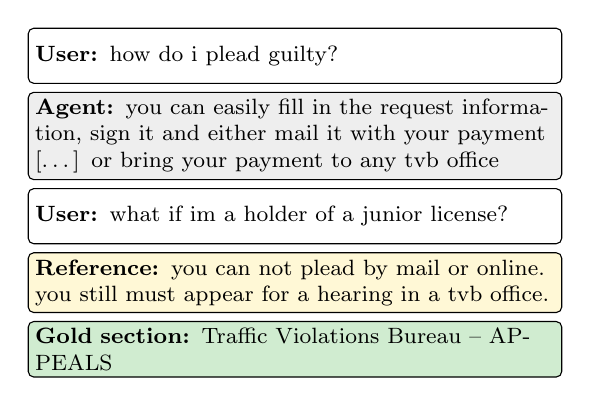
\begin{tikzpicture}[every node/.style={inner sep=3pt}]
  \tikzset{box/.append style={font=\footnotesize, align=left, text width=6.6cm}}
  \node[dat, rounded corners=2pt, fill=white] (a) {\textbf{User:} how do i plead guilty?};
  \node[dat, rounded corners=2pt, below=1mm of a] (b) {\textbf{Agent:} you can easily fill in the request information, sign it and either mail it with your payment [\ldots] or bring your payment to any tvb office};
  \node[dat, rounded corners=2pt, fill=white, below=1mm of b] (c) {\textbf{User:} what if im a holder of a junior license?};
  \node[prm, rounded corners=2pt, below=1mm of c] (d) {\textbf{Reference:} you can not plead by mail or online. you still must appear for a hearing in a tvb office.};
  \node[kg, rounded corners=2pt, below=1mm of d] (e) {\textbf{Gold section:} Traffic Violations Bureau -- APPEALS};
\end{tikzpicture}
\end{columns}
\end{frame}

% =====================================================================
\begin{frame}{Evaluation protocol}
\begin{columns}[T]
\column{0.5\textwidth}
\begin{itemize}
\item Token F1 per question (SQuAD normalisation), then the mean over questions
\item Reported on all, answerable and unanswerable questions; abstention recall and false abstention
\item Comparisons: paired bootstrap on the same questions, 95\% interval
\item An exact refusal on an unanswerable question scores F1 = 1
\end{itemize}
\column{0.46\textwidth}
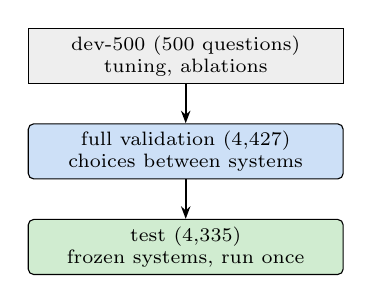
\begin{tikzpicture}[node distance=5mm]
  \node[dat, minimum width=40mm] (d) {dev-500 (500 questions)\\tuning, ablations}; % data/dev_500_ids.json
  \node[ret, below=of d, minimum width=40mm] (v) {full validation (4,427)\\choices between systems};
  \node[kg, below=of v, minimum width=40mm] (t) {test (4,335)\\frozen systems, run once};
  \draw[arr] (d) -- (v); \draw[arr] (v) -- (t);
\end{tikzpicture}
\end{columns}
\end{frame}

% =====================================================================
\begin{frame}{Baselines: lower and upper bound}
\begin{columns}[T]
\column{0.5\textwidth}
\begin{itemize}
\item \textbf{LLM only}: the user turn, no documents
\item \textbf{Oracle}: the gold sections given directly to the generator
\item Every retrieval system sits between the two
\end{itemize}
\column{0.46\textwidth}
\centering
\begin{tabular}{lcc}
\toprule
F1 (\%) & validation & test \\
\midrule
LLM only & 15.8 & 15.1 \\ % experiments/results/validation/diagnostics.md, experiments/results/test/diagnostics.md
Oracle & 35.5 & 34.2 \\ % experiments/results/validation/diagnostics.md, experiments/results/test/diagnostics.md
\midrule
\multicolumn{3}{l}{\footnotesize false abstention: LLM only 8.1 / 11.8\%,} \\ % experiments/results/validation/diagnostics.md, experiments/results/test/diagnostics.md
\multicolumn{3}{l}{\footnotesize oracle 2.0 / 2.4\%} \\ % experiments/results/validation/diagnostics.md, experiments/results/test/diagnostics.md
\bottomrule
\end{tabular}
\end{columns}
\end{frame}

% =====================================================================
\begin{frame}{Passage RAG pipeline}
\centering
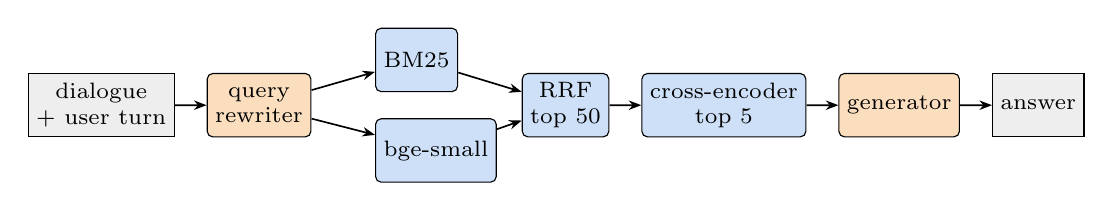
\begin{tikzpicture}[node distance=3.5mm, scale=1.15, transform shape]
  \node[dat] (h) {dialogue\\+ user turn};
  \node[llm, right=of h] (rw) {query\\rewriter};
  \node[ret, right=7mm of rw, yshift=5mm] (bm) {BM25};
  \node[ret, right=7mm of rw, yshift=-5mm] (de) {bge-small};
  \node[ret, right=7mm of bm, yshift=-5mm] (rrf) {RRF\\top 50};
  \node[ret, right=of rrf] (rr) {cross-encoder\\top 5};
  \node[llm, right=of rr] (g) {generator};
  \node[dat, right=of g] (a) {answer};
  \draw[arr] (h) -- (rw); \draw[arr] (rw) -- (bm); \draw[arr] (rw) -- (de);
  \draw[arr] (bm) -- (rrf); \draw[arr] (de) -- (rrf); \draw[arr] (rrf) -- (rr); \draw[arr] (rr) -- (g); \draw[arr] (g) -- (a);
\end{tikzpicture}

\vspace{4mm}
\small
\begin{tabular}{lcc}
\toprule
Full validation & F1 & R@5 \\
\midrule
LLM only & 15.8 & -- \\ % experiments/results/validation/diagnostics.md
BM25 & 24.1 & 40.6 \\ % experiments/results/rag_baseline_full_evaluation.json
Dense (bge-small) & 24.6 & 41.0 \\ % experiments/results/rag_dense_baseline_full_evaluation.json
Hybrid (RRF) & 24.7 & 44.7 \\ % experiments/results/rag_hybrid_baseline_full_evaluation.json
+ query rewriting & 26.8 & 59.4 \\ % experiments/results/rag_rewrite_baseline_full_evaluation.json
\midrule
+ agent prompt$^{*}$ & 26.5 & 59.8 \\ % experiments/results/validation/diagnostics.md
+ cross-encoder reranker & \up{26.9} & \up{63.7} \\ % experiments/results/validation/diagnostics.md
\bottomrule
\end{tabular}

\vspace{1mm}
{\scriptsize $^{*}$ second full-split run: the rewrites were regenerated (the LLM is not deterministic), so R@5 differs slightly from the row above.}
\end{frame}

% =====================================================================
\begin{frame}{Query rewriting}
\begin{columns}[T]
\column{0.48\textwidth}
\begin{itemize}
\item One LLM call per follow-up turn: last 6 turns + user turn $\to$ a self-contained search query
\item Used only for retrieval
\item The largest single gain: F1 24.7 $\to$ 26.8, R@5 44.7 $\to$ 59.4 % experiments/results/rag_hybrid_baseline_full_evaluation.json, experiments/results/rag_rewrite_baseline_full_evaluation.json
\item Right domain in the top 5: 69.4 $\to$ 92.5\% % experiments/results/rag_hybrid_baseline_full_evaluation.json, experiments/results/rag_rewrite_baseline_full_evaluation.json (domain_recall)
\end{itemize}
\column{0.48\textwidth}
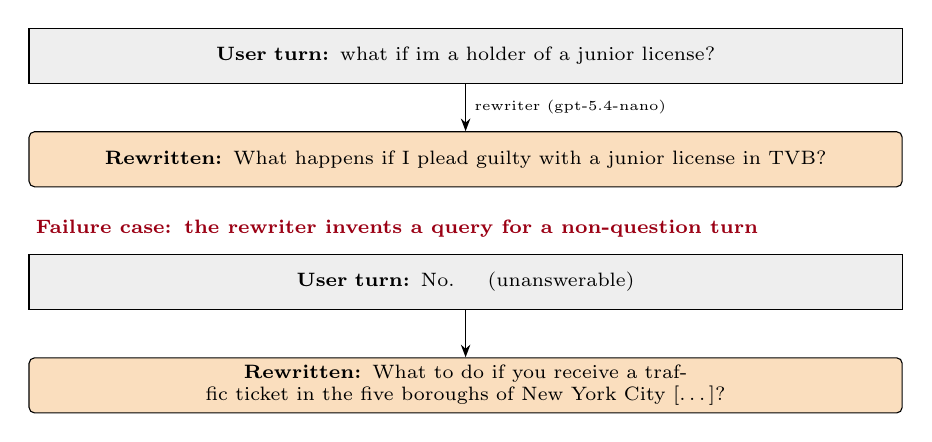
\begin{tikzpicture}[every node/.style={font=\scriptsize, align=left, text width=0.9\textwidth, inner sep=3pt}]
  \node[dat] (b) {\textbf{User turn:} what if im a holder of a junior license?};
  \node[llm, below=6mm of b, rounded corners=2pt] (a) {\textbf{Rewritten:} What happens if I plead guilty with a junior license in TVB?};
  \draw[arr] (b) -- node[right, font=\tiny, text width=3cm] {rewriter (\gen)} (a);
  \node[font=\scriptsize\bfseries, text=accent, below=3mm of a, anchor=north] (fl) {Failure case: the rewriter invents a query for a non-question turn};
  \node[dat, below=1mm of fl] (c) {\textbf{User turn:} No. \quad (unanswerable)};
  \node[llm, below=6mm of c, rounded corners=2pt] (d) {\textbf{Rewritten:} What to do if you receive a traffic ticket in the five boroughs of New York City [\ldots]?};
  \draw[arr] (c) -- (d);
\end{tikzpicture}
\end{columns}
\end{frame}

% =====================================================================
\begin{frame}{Knowledge graph construction}
\begin{columns}[c]
\column{0.56\textwidth}
\centering
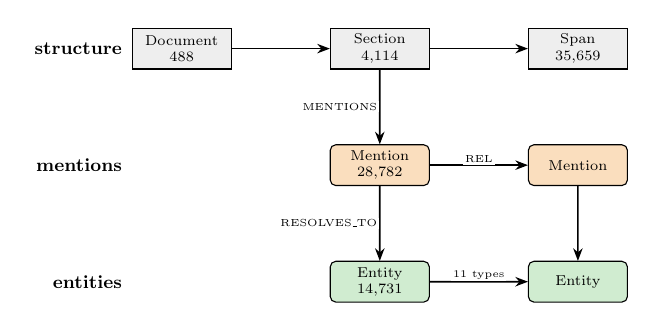
\begin{tikzpicture}[scale=0.74, transform shape]
  \node[dat, minimum width=17mm] (doc) at (0,0) {Document\\488};
  \node[dat, minimum width=17mm] (sec) at (3.4,0) {Section\\4,114};
  \node[dat, minimum width=17mm] (sp) at (6.8,0) {Span\\35,659};
  \draw[arr] (doc) -- (sec); \draw[arr] (sec) -- (sp);
  \node[box, fill=llmc, minimum width=17mm] (m1) at (3.4,-2) {Mention\\28,782};
  \node[box, fill=llmc, minimum width=17mm] (m2) at (6.8,-2) {Mention};
  \draw[arr] (sec) -- node[lab, left] {MENTIONS} (m1); \draw[arr] (m1) -- node[lab, above] {REL} (m2);
  \node[kg, minimum width=17mm] (e1) at (3.4,-4) {Entity\\14,731};
  \node[kg, minimum width=17mm] (e2) at (6.8,-4) {Entity};
  \draw[arr] (m1) -- node[lab, left] {RESOLVES\_TO} (e1); \draw[arr] (m2) -- (e2);
  \draw[arr] (e1) -- node[lab, above] {11 types} (e2);
  \node[font=\small\bfseries, anchor=east] at (-0.9,0) {structure};
  \node[font=\small\bfseries, anchor=east] at (-0.9,-2) {mentions};
  \node[font=\small\bfseries, anchor=east] at (-0.9,-4) {entities};
\end{tikzpicture}
% sizes: experiments/kg/full_build_report.md
\column{0.42\textwidth}
\begin{itemize}
\item Closed schema: 9 entity types, 11 relations with allowed type pairs % src/kg/schema.py
\item LLM extraction per section (JSON), then entity resolution with rules and an LLM judge
\item 13,277 typed relations, each with an evidence quote % experiments/kg/full_build_report.md
\item 16.2\% of the extracted relations broke the type rules % experiments/kg/full_build_report.md
\item Cost: 12,970 LLM calls, 22.2\,M input / 3.9\,M output tokens, about 1 hour, EUR 5--7 % experiments/kg/full_build_report.md; EUR from docs/schematic_report.tex (Cost section, derived from the Azure bill)
\end{itemize}
\end{columns}
\end{frame}

% =====================================================================
\begin{frame}{Graph quality}
\begin{columns}[T]
\column{0.5\textwidth}
\begin{itemize}
\item Control sample from the full graph: 22 of 30 triples correct, precision 73\% [56, 86] % experiments/kg/control_scores.json
\item Pilot on 3 annotated documents: precision 51\%, recall 66\% % experiments/kg/v1_v2_comparison.md
\item Not deterministic: two runs with the same settings share a third of their triples (Jaccard 0.33) % experiments/kg/pilot3_report.md
\item Entity and relation precision, separately, on 6 unseen documents: next slide
\end{itemize}
\column{0.46\textwidth}
\footnotesize
\textbf{Typical errors}\\[3pt]
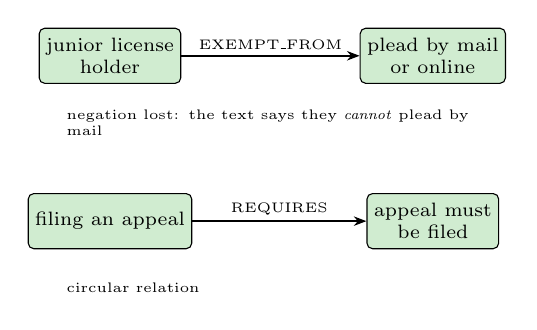
\begin{tikzpicture}[every node/.style={font=\scriptsize}]
  \node[kg] (jr) at (0,0) {junior license\\holder};
  \node[kg] (pm) at (4.1,0) {plead by mail\\or online};
  \draw[arr] (jr) -- node[lab, above=1pt] {EXEMPT\_FROM} (pm);
  \node[font=\tiny, text width=5.5cm, align=left] at (2.2,-0.85) {negation lost: the text says they \emph{cannot} plead by mail};
  \node[kg] (fa) at (0,-2.1) {filing an appeal};
  \node[kg] (mu) at (4.1,-2.1) {appeal must\\be filed};
  \draw[arr] (fa) -- node[lab, above=1pt] {REQUIRES} (mu);
  \node[font=\tiny, text width=5.5cm, align=left] at (2.2,-2.95) {circular relation};
\end{tikzpicture}
\end{columns}
\end{frame}

% =====================================================================
\begin{frame}{Extraction precision (Q9)}
\footnotesize
6 documents not used before (seeded, stratified by domain), labelled by hand with fixed guidelines; Wilson 95\% intervals % experiments/kg_eval/precision_scores.json, experiments/kg_eval/docs.json
\vspace{1mm}

\begin{columns}[T]
\column{0.42\textwidth}
\centering
\vspace{2mm}
\begin{tabular}{@{}lrr@{}}
\toprule
 & Entities & Relations \\
\midrule
Labelled & 150 & 115 \\
Correct & 87 & 90 \\
Precision & \textbf{58.0\%} & \textbf{78.3\%} \\
95\% CI & [50.0, 65.6] & [69.9, 84.8] \\
\bottomrule
\end{tabular}

\vspace{2mm}
\raggedright\scriptsize
Entities: a seeded sample of 150 of the 159 in the 6 documents. Relations: all 115.
\column{0.54\textwidth}
\textbf{Errors per type}\\[2pt]
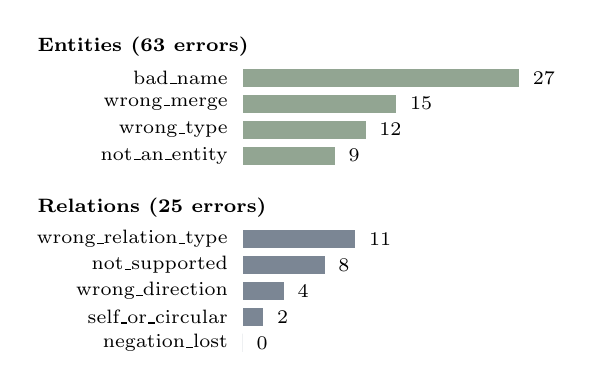
\begin{tikzpicture}[x=1.3mm, y=3.3mm, every node/.style={font=\scriptsize}]
  \foreach \lab/\n/\y in {bad\_name/27/0, wrong\_merge/15/1, wrong\_type/12/2, not\_an\_entity/9/3} {
    \fill[kgc!70!black] (0,-\y-0.35) rectangle (\n,-\y+0.35);
    \node[anchor=east] at (-0.5,-\y) {\lab};
    \node[anchor=west] at (\n+0.4,-\y) {\n};
  }
  \node[anchor=west, font=\scriptsize\bfseries] at (-21,1.2) {Entities (63 errors)};
  \foreach \lab/\n/\y in {wrong\_relation\_type/11/6.2, not\_supported/8/7.2, wrong\_direction/4/8.2, self\_or\_circular/2/9.2, negation\_lost/0/10.2} {
    \fill[retc!60!black] (0,-\y-0.35) rectangle (\n,-\y+0.35);
    \node[anchor=east] at (-0.5,-\y) {\lab};
    \node[anchor=west] at (\n+0.4,-\y) {\n};
  }
  \node[anchor=west, font=\scriptsize\bfseries] at (-21,-5) {Relations (25 errors)};
\end{tikzpicture}
\end{columns}

\vspace{1mm}
\small
Few invented facts (7\% of relations unsupported, 6\% of entities not real); main problems are names, merges and relation type.

\vspace{1mm}
\scriptsize\color{muted}
Not comparable to the earlier 30-triple check (whole triples, other documents and rules).
\end{frame}

% =====================================================================
\begin{frame}{Using the graph}
\begin{itemize}
\item Entity linking: the rewritten query $\to$ 10 entities (BM25 + embeddings over names); an entity of the gold section is among them for 70\% of dev-500 % experiments/kg_rag/phase2_report.md
\end{itemize}
\vspace{2mm}
\centering
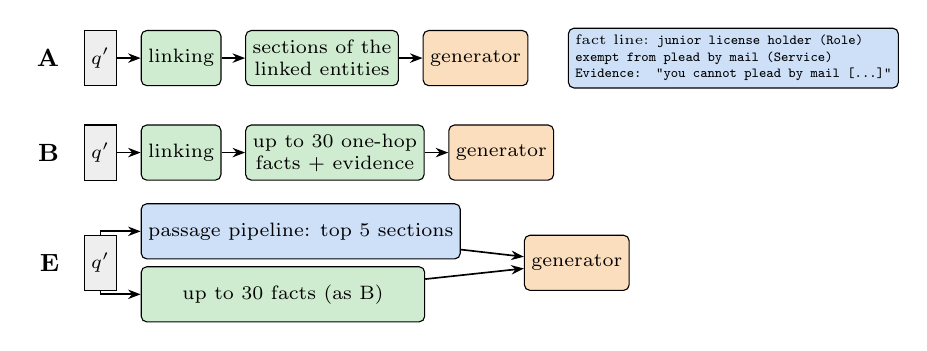
\begin{tikzpicture}[node distance=3mm]
  \node[font=\small\bfseries, anchor=east] at (-0.4,0) {A};
  \node[dat] (q1) at (0,0) {$q'$};
  \node[kg, right=of q1] (l1) {linking};
  \node[kg, right=of l1] (s1) {sections of the\\linked entities};
  \node[llm, right=of s1] (g1) {generator};
  \draw[arr] (q1) -- (l1); \draw[arr] (l1) -- (s1); \draw[arr] (s1) -- (g1);
  \node[font=\small\bfseries, anchor=east] at (-0.4,-1.2) {B};
  \node[dat] (q2) at (0,-1.2) {$q'$};
  \node[kg, right=of q2] (l2) {linking};
  \node[kg, right=of l2] (f2) {up to 30 one-hop\\facts + evidence};
  \node[llm, right=of f2] (g2) {generator};
  \draw[arr] (q2) -- (l2); \draw[arr] (l2) -- (f2); \draw[arr] (f2) -- (g2);
  \node[font=\small\bfseries, anchor=east] at (-0.4,-2.6) {E};
  \node[dat] (q3) at (0,-2.6) {$q'$};
  \node[ret, right=of q3, yshift=4mm] (p3) {passage pipeline: top 5 sections};
  \node[kg, right=of q3, yshift=-4mm, minimum width=36mm] (f3) {up to 30 facts (as B)};
  \node[llm, right=8mm of p3, yshift=-4mm] (g3) {generator};
  \draw[arr] (q3) |- (p3); \draw[arr] (q3) |- (f3); \draw[arr] (p3) -- (g3); \draw[arr] (f3) -- (g3);
  \node[ret, right=5mm of g1, font=\tiny, align=left] {fact line: \texttt{junior license holder (Role)}\\\texttt{exempt from plead by mail (Service)}\\\texttt{Evidence: "you cannot plead by mail [\ldots]"}};
\end{tikzpicture}

\vspace{2mm}
\raggedright\footnotesize
Local, entity-centric Graph RAG (graph facts added to passage retrieval). Global community summaries (GraphRAG-style) were not used: MultiDoc2Dial questions are local to one section.
\end{frame}

% =====================================================================
\begin{frame}{Graph results and the random-facts control}
\centering
\small
\begin{tabular}{lccccc}
\toprule
& \multicolumn{3}{c}{validation} & \multicolumn{2}{c}{test} \\
F1 (\%) & all & answerable & R@5 & all & answerable \\
\midrule
Passages & 26.9 & 27.2 & 63.7 & 26.9 & 27.1 \\ % experiments/results/validation/kg_qa_summary.json, experiments/results/test/kg_qa_summary.json
A: graph sections & \down{23.0} & 22.4 & 34.0 & \multicolumn{2}{c}{\footnotesize not run} \\ % experiments/results/validation/kg_qa_summary.json
B: graph facts & \down{24.1} & 23.8 & 36.6 & 23.8 & 23.3 \\ % experiments/results/validation/kg_qa_summary.json, experiments/results/test/kg_qa_summary.json
E: passages + facts & 27.4 & \up{27.7} & 63.7 & 27.5 & \up{28.0} \\ % experiments/results/validation/kg_qa_summary.json, experiments/results/test/kg_qa_summary.json
E with random facts & 27.4 & 27.2 & 63.7 & 27.3 & 27.1 \\ % experiments/results/validation/kg_qa_summary.json, experiments/results/test/kg_qa_summary.json
\bottomrule
\end{tabular}

\vspace{4mm}
\begin{itemize}
\item Generator sees the user turn only (G0); the dialogue history comes on slide 11
\item The graph alone ranks sections badly: R@5 half of passage retrieval
\item Facts added to passages help on answerable questions; random facts do not (they only make the model abstain more)
\end{itemize}
\end{frame}

% =====================================================================
\begin{frame}[label=conv]{Conversational generator}
\begin{columns}[c]
\column{0.44\textwidth}
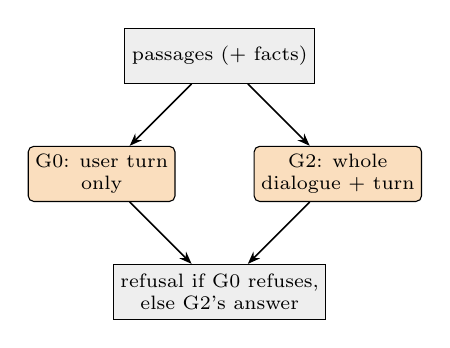
\begin{tikzpicture}
  \node[dat] (c) at (0,0) {passages (+ facts)};
  \node[llm] (g0) at (-1.5,-1.5) {G0: user turn\\only};
  \node[llm] (g2) at (1.5,-1.5) {G2: whole\\dialogue + turn};
  \node[dat] (a) at (0,-3.0) {refusal if G0 refuses,\\else G2's answer};
  \draw[arr] (c) -- (g0); \draw[arr] (c) -- (g2); \draw[arr] (g0) -- (a); \draw[arr] (g2) -- (a);
\end{tikzpicture}
\column{0.53\textwidth}
\small
\begin{tabular}{lccc}
\toprule
Passages + facts & all & answ. & unansw. \\
\midrule
G0 (user turn only) & 27.4 & 27.7 & 20.1 \\ % experiments/results/validation/generator_input/summary.md
G2 (with dialogue) & 27.7 & \up{28.5} & \down{12.9} \\ % experiments/results/validation/generator_input/summary.md
G2 + abstain(G0) & \up{28.0} & 28.2 & 24.5 \\ % experiments/results/validation/generator_input/summary.md
\bottomrule
\end{tabular}

\vspace{3mm}
\footnotesize
\begin{itemize}
\item The history helps on turns like ``yes'' (+3.2) but halves abstention % experiments/results/validation/generator_input/summary.md
\item Cheaper decisions lose: yes/no classifier $-1.0$, reranker threshold $-0.6$ % experiments/results/validation/generator_input/abstention_decision.md
\end{itemize}
\end{columns}
\end{frame}

% =====================================================================
\begin{frame}[label=graphhelp]{When does the graph help?}
\centering
\small
\begin{tabular}{lrccc}
\toprule
Validation & $n$ & passages & + facts & $d$ [95\% CI] \\
\midrule
All questions & 4,427 & 27.5 & 28.0 & +0.5 [0.1, 0.9] \\ % experiments/results/validation/graph_analysis/summary.md
Passages miss, a fact from gold & 342 & 20.6 & 25.2 & \up{+4.6} [2.7, 6.6] \\ % experiments/results/validation/graph_analysis/summary.md
Passages hit, no fact from gold & 1,005 & 31.9 & 30.9 & \down{$-1.0$} [$-1.9$, $-0.1$] \\ % experiments/results/validation/graph_analysis/summary.md
\bottomrule
\end{tabular}

\vspace{5mm}
\begin{itemize}
\item Oracle router (better system per question): +3.3 F1; the better of two runs of the \emph{same} system already gives +2.9 % experiments/results/validation/graph_analysis/summary.md
\item A router on pre-generation signals is right 52\% of the time and loses 0.5 F1 $\Rightarrow$ not worth it % experiments/results/validation/graph_analysis/summary.md
\end{itemize}
\end{frame}

% =====================================================================
\begin{frame}{Graph RAG variants}
\small
\renewcommand{\arraystretch}{1.25}
\begin{tabular}{>{\raggedright}p{4.3cm}>{\raggedright\arraybackslash}p{8.3cm}}
\toprule
Variant & Outcome (validation) \\
\midrule
V1: top 10 facts by cross-encoder score & same F1 as 30 facts (28.0) with 35\% fewer input tokens; cuts the facts that rescue misses ($-2.0$ on the 342) \\ % experiments/results/validation/graph_rag/summary.md
\midrule
V2: facts from outside the top 5 first & recovers the misses (+2.4 on the 342 vs V1), no gain overall \\ % experiments/results/validation/graph_rag/summary.md
\midrule
V3: graph score as reranker signal & R@5 falls for every weight $> 0$, from 67.8 down to 54.6 at weight 2 (dev-500); not used \\ % experiments/results/validation/graph_rag/v3_retrieval.md
\midrule
V4: two-hop paths & reach no gold section that one-hop facts miss (0\%); dropped \\ % experiments/results/validation/graph_rag/decisions.md
\bottomrule
\end{tabular}

\vspace{4mm}
\normalsize
All variants tuned on dev-500 with stopping rules fixed in advance. Only top-10 facts (V1) went to the test split, together with P and E.
\end{frame}

% =====================================================================
\begin{frame}{Agents}
\centering
\footnotesize
\renewcommand{\arraystretch}{1.25}
\begin{tabular}{lccc}
\toprule
 & $\Delta$ F1 all & $\Delta$ F1 answerable & USD / 1,000 turns \\
\midrule
E: passages + 30 facts & --- & --- & 1.39 \\ % experiments/results/dev_500/agent/a1_summary.json
A1: check + one extra round & $-0.6$ [$-1.6$, 0.4] & $+0.1$ [$-0.5$, 0.6] & 2.29 ($+65\%$) \\ % experiments/results/dev_500/agent/a1_summary.json
A2: tools, own refusal & $-2.8$ [$-4.5$, $-1.3$] & $-0.5$ [$-1.6$, 0.6] & 1.23 ($-12\%$) \\ % experiments/results/dev_500/agent/a2_summary.json
\bottomrule
\end{tabular}

\vspace{4mm}
\footnotesize dev-500, against E with citations; the check separates the questions (J = 0.33) but neither agent beat E, so neither went to the full validation split.

\vspace{4mm}
\normalsize
The model can tell when the context is missing, but a second search or tool calls do not recover the gold section often enough, and an agent that refuses on its own almost never does.
\end{frame}

% =====================================================================
\begin{frame}{Generator models and cost}
\centering
\footnotesize
\begin{tabular}{lccccc}
\toprule
 & & & false & tokens / turn & USD per \\
Generator & F1 all & answ. & abstention & in / out (reasoning) & 1,000 conv. \\
\midrule
\gen{}$^{*}$ & 28.1 & \up{28.4} & 3.9\% & 5,793 / 106 (0) & 7.30 \\ % experiments/results/validation/model_comparison/summary.md
gpt-5-nano & 28.1 & 26.8 & 11.6\% & 5,532 / 1,578 (1,435) & 5.94 \\ % experiments/results/validation/model_comparison/summary.md
gpt-6-luna & 27.3 & 26.6 & 14.2\% & 5,511 / 176 (102) & 3.89 \\ % experiments/results/validation/model_comparison/summary.md
\bottomrule
\end{tabular}

\vspace{4mm}
\begin{itemize}
\item Where all three answer, F1 is the same (30.8 / 30.7 / 30.8): newer models refuse more, they do not answer worse % experiments/results/validation/model_comparison/summary.md
\item gpt-5-nano spends about 1,400 hidden reasoning tokens per turn % experiments/results/validation/model_comparison/summary.md
\item Passages + facts with dialogue history, validation; USD list prices (Azure Retail Prices API) % experiments/results/validation/model_comparison/summary.md
\end{itemize}

\vspace{1mm}
{\scriptsize $^{*}$ re-run with API usage logging; differs from the cached run (slides \ref{conv}, \ref{graphhelp}, \ref{backval}: 28.0 / 28.2) by 0.1--0.2 F1.}
\end{frame}

% =====================================================================
\begin{frame}{Final results on the test split}
\centering
\begin{tabular}{lccc}
\toprule
Test, 4,335 questions & F1 all & answerable & input tokens / turn \\
\midrule
LLM only & 15.1 & 15.0 & 65 \\ % experiments/results/test/baselines_by_answerability.json, docs/schematic/token_estimates_test.json
P: passages & 27.6 & 27.5 & 2,324 \\ % experiments/results/test/step7_final.md
E: passages + 30 facts & \up{28.2} & \up{28.4} & 5,621 \\ % experiments/results/test/step7_final.md
V1: passages + top 10 facts & 27.8 & 28.1 & 3,608 \\ % experiments/results/test/step7_final.md
Oracle & 34.2 & 35.1 & 456 \\ % experiments/results/test/baselines_by_answerability.json, docs/schematic/token_estimates_test.json
\bottomrule
\end{tabular}

\vspace{4mm}
\begin{itemize}
\item P, E, V1 with dialogue history and the separate abstention decision (two generator calls); LLM only and oracle with the user turn only (one call)
\item E vs P: +0.6 [0.1, 1.0] all, +0.9 [0.6, 1.2] answerable; V1 vs E: $-0.4$ [$-0.7$, 0.0] % experiments/results/test/step7_final.md
\end{itemize}
\end{frame}

% =====================================================================
\begin{frame}{LLM judge}
\small
\begin{itemize}
\item gpt-6-luna rates each answer correct / partial / incorrect against the reference and the gold section (citations stripped, abstentions by rule); score 1 / 0.5 / 0
\item Human check on 60 answers of P, E, V1: $\kappa$ = 0.65 (3 classes), 90\% agreement on correct+partial vs incorrect; the judge is stricter than the human % experiments/results/judge/gpt-6-luna/dev_500/human_agreement.json
\end{itemize}

\vspace{2mm}
\centering
\begin{tabular}{lcc}
\toprule
Test & judge score & F1 all \\
\midrule
P: passages & 67.3 & 27.6 \\ % experiments/results/judge/gpt-6-luna/test/summary.md
E: passages + 30 facts & \up{68.5} & \up{28.2} \\ % experiments/results/judge/gpt-6-luna/test/summary.md
V1: passages + top 10 facts & 67.3 & 27.8 \\ % experiments/results/judge/gpt-6-luna/test/summary.md
\midrule
E vs P & $+1.3$ [0.3, 2.2] & $+0.6$ [0.2, 1.0] \\ % experiments/results/judge/gpt-6-luna/test/summary.md
V1 vs E & $-1.2$ [$-2.0$, $-0.4$] & $-0.4$ [$-0.7$, 0.0] \\ % experiments/results/judge/gpt-6-luna/test/summary.md
\bottomrule
\end{tabular}

\vspace{2mm}
\raggedright\scriptsize Paired over the 4,334 test questions with a verdict (one blocked by the content filter). Judge and generator are from the same model family. Evaluation only: no system re-selected.
\end{frame}

% =====================================================================
\begin{frame}{Why F1 is not enough}
\footnotesize
\begin{columns}[T]
\column{0.48\textwidth}
\textbf{Correct answer, F1 near 0} % experiments/results/judge/gpt-6-luna/dev_500/human_labels.csv (h018)
\par\vspace{2pt}
\textbf{User:} I need information from Proof of Supplemental Security Income\\[3pt]
\textbf{Answer:} To prove you receive SSI at the DMV, bring an original Notice of Award, COLA letter, SSA-2258 benefit verification letter [\ldots]\\[3pt]
\textbf{Reference:} you receive SSI?\\[3pt]
\textbf{F1} 0.11 \quad \textbf{judge / human:} correct / correct
\column{0.48\textwidth}
\textbf{Dataset noise} % experiments/results/judge/gpt-6-luna/dev_500/human_labels.csv (h004)
\par\vspace{2pt}
\textbf{User} (after VA homelessness help): Where can I get more information?\\[3pt]
\textbf{Answer:} Call the VA hotline 800-827-1000, or the National Call Center for Homeless Veterans [\ldots]\\[3pt]
\textbf{Reference:} Learn about suicide prevention [\ldots] Visit our suicide prevention website\\[3pt]
\textbf{F1} 0.15 \quad \textbf{judge / human:} incorrect / incorrect
\end{columns}

\vspace{3mm}
\small The reference is a clarifying question in the first case; in the second the gold turn switches to a topic the user never raised, so a reasonable answer to the conversation is scored wrong by both measures.
\end{frame}

% =====================================================================
\begin{frame}{Sources per answer}
\begin{columns}[T]
\column{0.44\textwidth}
\footnotesize
\begin{tabular}{lc}
\toprule
Answered (validation) & first source gold \\
\midrule
all & 42.2\% \\ % experiments/results/validation/sources/cite_validation.json
gold in the top 5 & 63.4\% \\ % experiments/results/validation/sources/cite_validation.json
gold not retrieved & \phantom{0}2.6\% \\ % experiments/results/validation/sources/cite_validation.json
\bottomrule
\end{tabular}

\vspace{3mm}
\small
\begin{itemize}
\item The answer ends with the passages and facts it used: [2], [F7]
\item Citations cost no quality: F1 +0.3 [0.0, 0.6], +56 tokens per answer % experiments/results/validation/sources/cite_validation.json (50 input + 6 output tokens)
\end{itemize}
\column{0.52\textwidth}
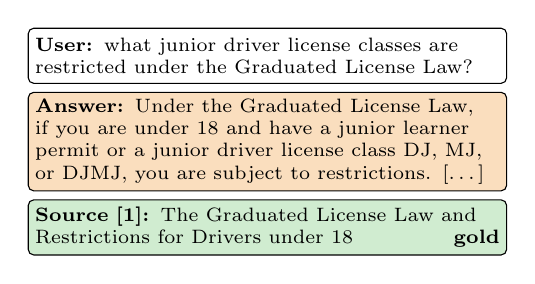
\begin{tikzpicture}[every node/.style={inner sep=3pt}]
  \tikzset{box/.append style={font=\scriptsize, align=left, text width=5.9cm}}
  \node[dat, rounded corners=2pt, fill=white] (q) {\textbf{User:} what junior driver license classes are restricted under the Graduated License Law?}; % experiments/results/validation/sources/demo_examples.md (example 4)
  \node[llm, rounded corners=2pt, below=1mm of q] (a) {\textbf{Answer:} Under the Graduated License Law, if you are under 18 and have a junior learner permit or a junior driver license class DJ, MJ, or DJMJ, you are subject to restrictions. [\ldots]};
  \node[kg, rounded corners=2pt, below=1mm of a] (s) {\textbf{Source [1]:} The Graduated License Law and Restrictions for Drivers under 18 \hfill \textbf{gold}};
\end{tikzpicture}
\end{columns}
\end{frame}

% =====================================================================
\begin{frame}{Conclusions}
\begin{itemize}
\setlength{\itemsep}{6pt}
\item Retrieval is the main lever: query rewriting gave the largest gain, and answers are much better when the gold section is retrieved (test F1 31.9 on hits, 17.4 on misses) % experiments/results/test/diagnostics.md
\item The knowledge graph alone is worse than passages; its facts added to the passages give a small, consistent gain on answerable questions (+0.9 on test) % experiments/results/test/step7_final.md
\item The gain comes from a small group of questions (passages miss, a fact points to the right section) that cannot be identified before generation
\item E is best under both measures on test: F1 $+0.6$ [0.2, 1.0], judge $+1.3$ [0.3, 2.2] vs P % experiments/results/judge/gpt-6-luna/test/summary.md
\item Top-10 facts save 36\% input tokens but cost quality on test (F1 $-0.4$ [$-0.7$, 0.0], judge $-1.2$ [$-2.0$, $-0.4$] vs E); on validation the judge shows no difference % experiments/results/judge/gpt-6-luna/test/summary.md, experiments/results/judge/gpt-6-luna/validation/summary.md
\item With the dialogue history the generator answers better but must decide separately whether to refuse; \gen{} stays the generator
\end{itemize}
\end{frame}

% =====================================================================
\begin{frame}{Demo}
\small Local Gradio chat over the final E pipeline; prompts identical to the evaluated system (194/194 replay checks) % demo/check_replay.py
\vspace{1mm}

\centering
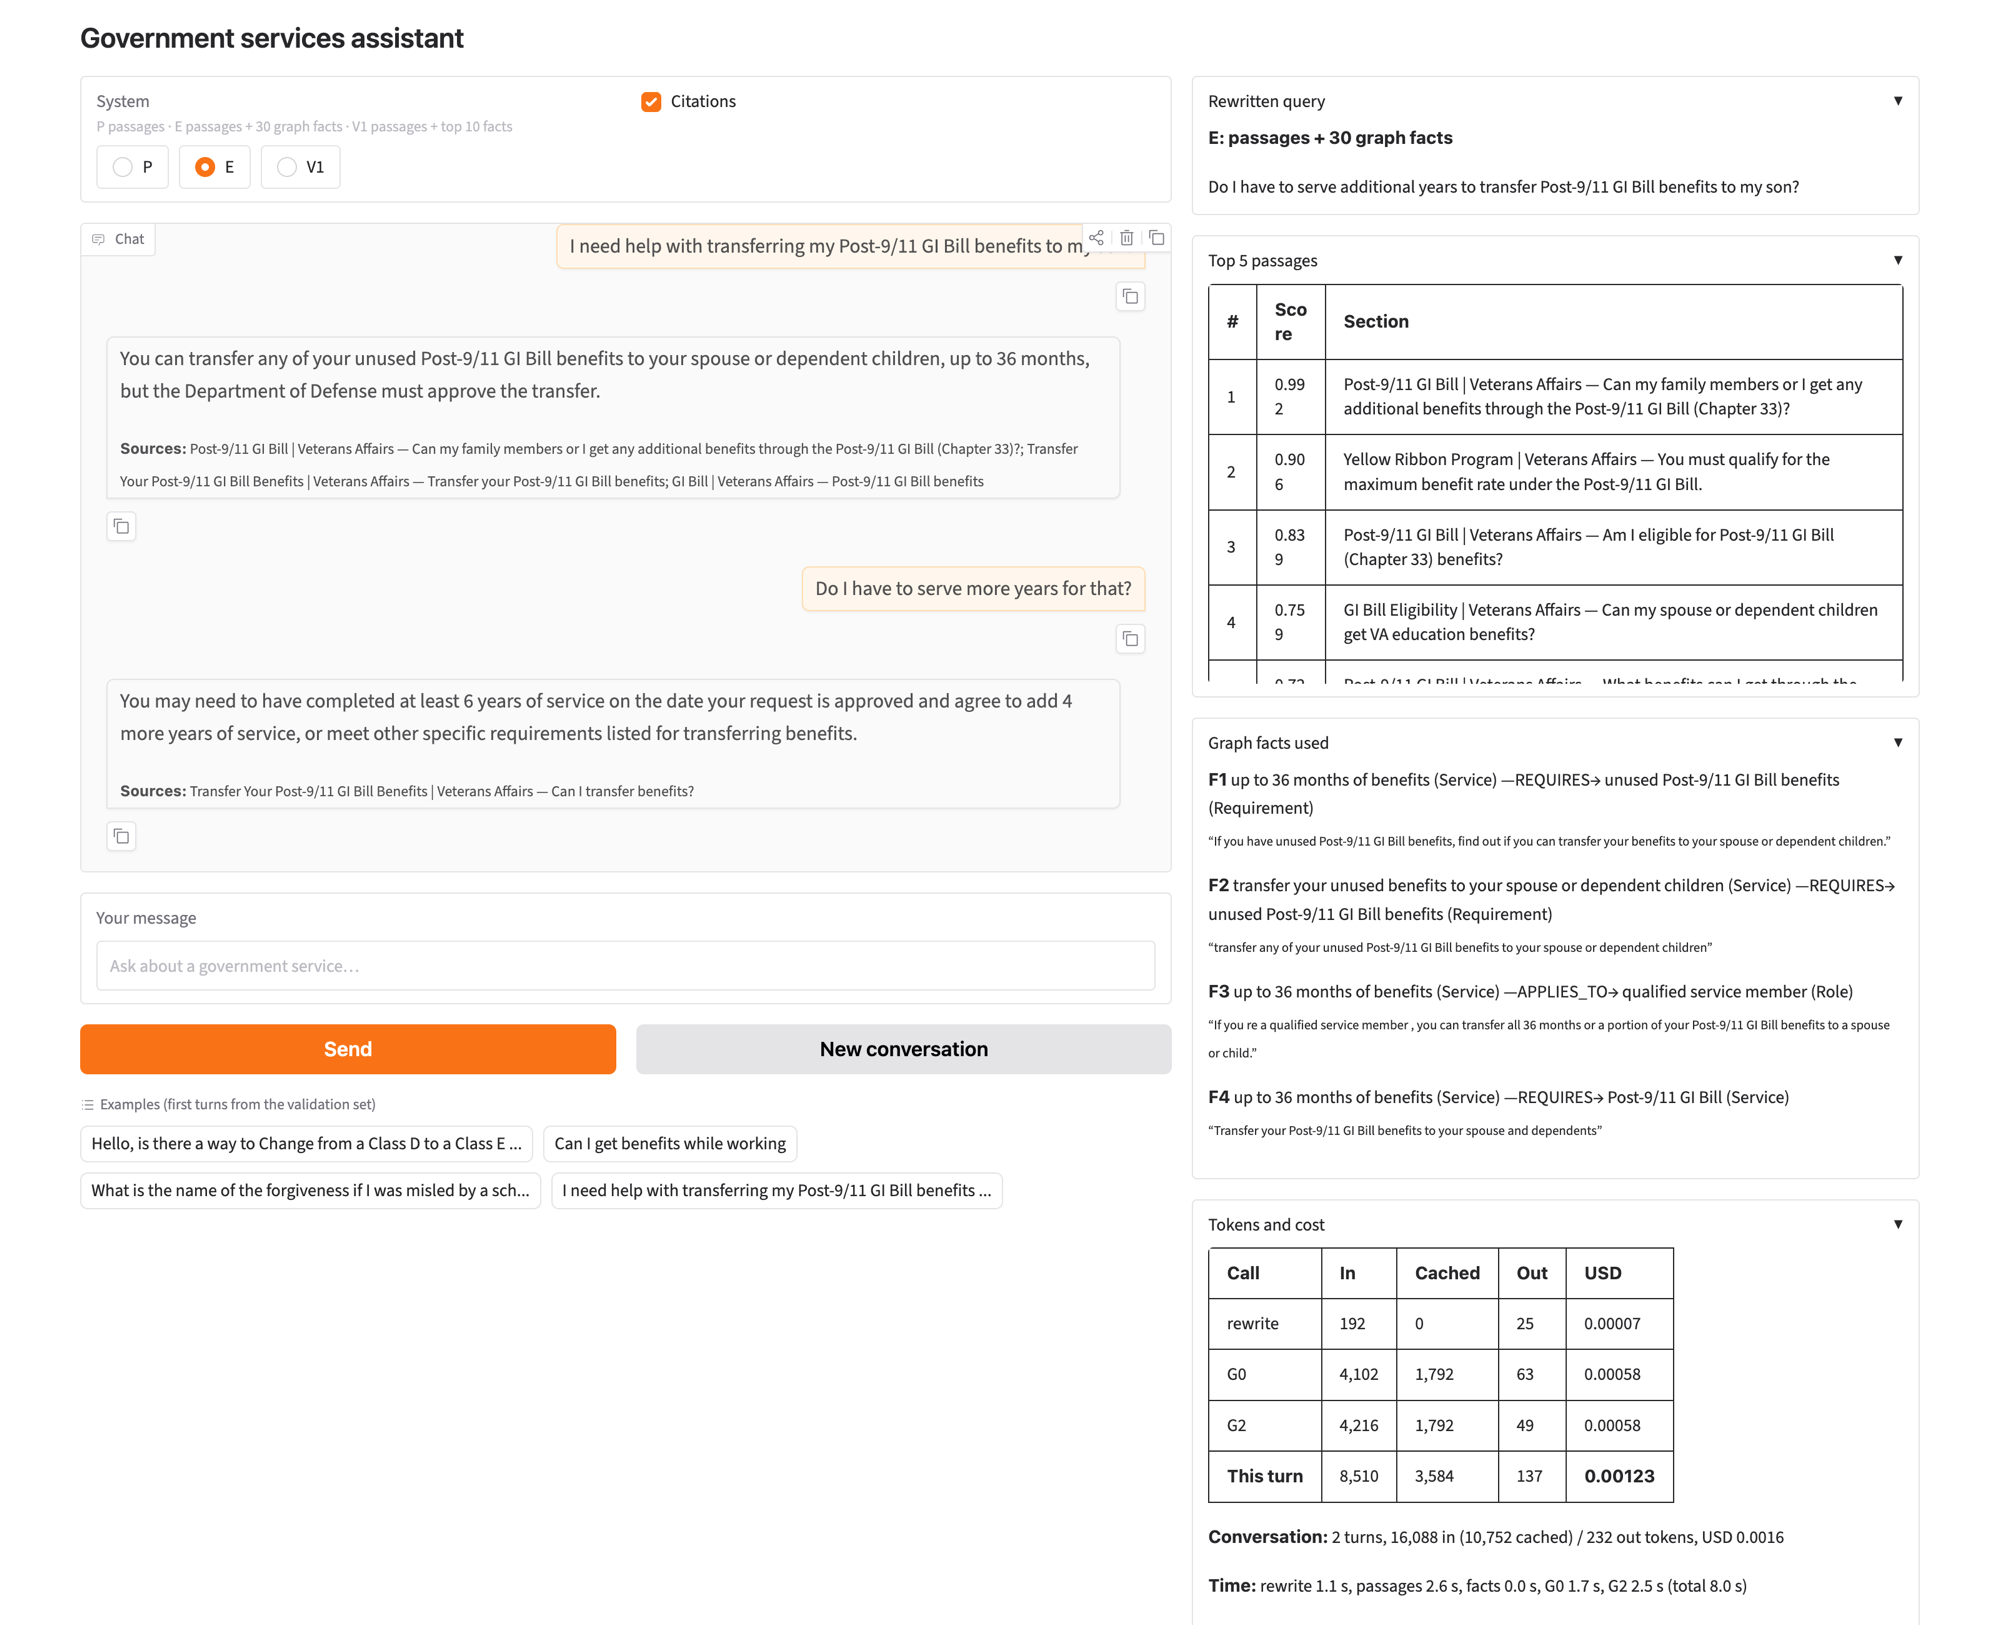
\includegraphics[height=0.77\textheight]{figures/demo.png}
\end{frame}

% =====================================================================
\begin{frame}{Open items and next steps}
\begin{itemize}
\setlength{\itemsep}{5pt}
\item Error analysis of the final systems
\item Agent with a second retrieval round: ranks 6--10 of the first list plus a separate refusal decision (future work from the agent experiments)
\item Report writing
\item EnronQA and MTRAG datasets
\end{itemize}
\end{frame}

% =====================================================================
\begin{frame}[label=backval]{Backup: validation}
\centering
\footnotesize
\begin{tabular}{lcccccc}
\toprule
Full validation (4,427) & F1 all & answ. & unansw. & R@5 & abstain recall & false abst. \\
\midrule
LLM only & 15.8 & 15.7 & 18.4 & -- & 17.3 & 8.1 \\ % experiments/results/validation/baselines_by_answerability.json
Passages & 26.9 & 27.2 & 20.2 & 63.7 & 19.5 & 4.5 \\ % experiments/results/validation/kg_qa_summary.json, experiments/results/validation/diagnostics.md
A: graph sections & 23.0 & 22.4 & 32.5 & 34.0 & 32.3 & 10.4 \\ % experiments/results/validation/kg_qa_summary.json, experiments/results/validation/diagnostics.md
B: graph facts & 24.1 & 23.8 & 30.6 & 36.6 & 30.1 & 7.6 \\ % experiments/results/validation/kg_qa_summary.json, experiments/results/validation/diagnostics.md
E: passages + facts & 27.4 & 27.7 & 20.1 & 63.7 & 19.0 & 3.4 \\ % experiments/results/validation/kg_qa_summary.json, experiments/results/validation/diagnostics.md
E-random & 27.4 & 27.2 & 31.9 & 63.7 & 31.4 & 5.6 \\ % experiments/results/validation/kg_qa_summary.json, experiments/results/validation/diagnostics.md
Oracle & 35.5 & 36.5 & 15.9 & 100 & 15.5 & 2.0 \\ % experiments/results/validation/baselines_by_answerability.json
\midrule
\multicolumn{7}{l}{\emph{with dialogue history (G2 + abstain(G0))}} \\
Passages & 27.5 & 27.6 & 24.6 & 63.7 & 24.3 & 5.6 \\ % experiments/results/validation/generator_input/summary.md; R@5: experiments/results/validation/diagnostics.md
Passages + 30 facts & 28.0 & 28.2 & 24.5 & 63.7 & 23.5 & 4.6 \\ % experiments/results/validation/generator_input/summary.md; R@5: experiments/results/validation/diagnostics.md
Passages + top 10 facts & 28.0 & 28.3 & 22.5 & 63.7 & 21.2 & 3.9 \\ % experiments/results/validation/graph_rag/summary.md; R@5: experiments/results/validation/diagnostics.md
Graph facts only & 24.6 & 24.1 & 33.9 & 36.6 & 33.2 & 10.0 \\ % experiments/results/validation/graph_rag/summary.md; R@5: experiments/results/validation/diagnostics.md (kg_facts, same retrieval)
\bottomrule
\end{tabular}
\end{frame}

% =====================================================================
\begin{frame}{Backup: test}
\centering
\footnotesize
\begin{tabular}{lcccccc}
\toprule
Test (4,335) & F1 all & answ. & unansw. & R@5 & abstain recall & false abst. \\
\midrule
LLM only & 15.1 & 15.0 & 15.7 & -- & 14.5 & 11.8 \\ % experiments/results/test/baselines_by_answerability.json
Passages & 26.9 & 27.1 & 23.3 & 66.6 & 22.4 & 5.2 \\ % experiments/results/test/kg_qa_summary.json, experiments/results/test/diagnostics.md
B: graph facts & 23.8 & 23.3 & 32.6 & 38.7 & 32.0 & 10.0 \\ % experiments/results/test/kg_qa_summary.json, experiments/results/test/diagnostics.md
E: passages + facts & 27.5 & 28.0 & 20.4 & 66.6 & 19.1 & 3.3 \\ % experiments/results/test/kg_qa_summary.json, experiments/results/test/diagnostics.md
E-random & 27.3 & 27.1 & 30.9 & 66.6 & 29.9 & 6.5 \\ % experiments/results/test/kg_qa_summary.json, experiments/results/test/diagnostics.md
Oracle & 34.2 & 35.1 & 19.6 & 100 & 18.7 & 2.4 \\ % experiments/results/test/baselines_by_answerability.json
\midrule
\multicolumn{7}{l}{\emph{with dialogue history (G2 + abstain(G0))}} \\
Passages & 27.6 & 27.5 & 28.4 & 66.6 & 27.4 & 6.3 \\ % experiments/results/test/step7_final.md, experiments/results/test/diagnostics.md (R@5)
Passages + 30 facts & 28.2 & 28.4 & 24.1 & 66.6 & 23.7 & 4.4 \\ % experiments/results/test/step7_final.md; R@5: experiments/results/test/diagnostics.md
Passages + top 10 facts & 27.8 & 28.1 & 22.3 & 66.6 & 21.6 & 4.5 \\ % experiments/results/test/step7_final.md; R@5: experiments/results/test/diagnostics.md
\bottomrule
\end{tabular}
\end{frame}

\end{document}
